\section{Исследование и построение решения задачи}
\label{sec:Section3} \index{Section3}

\subsection{Устройство архитектуры системы процессор-память}

\subsubsection{Микроархитектура процессора}

    Современный ЦП (центральный процессор) представляет собой
    систему взаимосвязанных между собой процессорных ядер, не обязательно одинаковых.

    Исполнение инструкции современным процессорным ядром является многостадийным конвейером
    из различных блоков. В зависимости от исполняемой рабочей нагрузки утилизируются различные блоки
    процессора, поэтому скорость исполнения таковой рабочей нагрузки сильно зависит
    от её особенностей (типа) и особенностей исполнения таковых нагрузок на блоках процессора.

    В наиболее общем виде можно разбить конвейер исполнения инструкции на процессоре на несколько
    последовательных стадий:
    \begin{enumerate}
        \item Чтение инструкции из памяти;
        \item Декодирование прочитанной инструкции;
        \item Исполнение инструкции на вычислительных блоках;
        \item Чтение/запись в память при необходимости;
        \item Запись результата исполнения инструкции в регистры процессора.
    \end{enumerate}

    Чаще всего приведённые выше стадии дробятся на несколько более узконаправленных стадий, применяются
    дополнительные оптимизации для ускорения исполнения инструкций а также их распараллеливания
    (например, кеширование декодированных инструкций и предсказатель ветвлений). Наиболее
    актуальным примером являются ядра процессора с маханизмом спекулятивного (внеочередного) выполнения
    инструкций (Out-of-Order), в которых используется алгоритм Томасуло, позволяющий реализовать
    исполнение машинных инструкций не в порядке их следования в машинном коде, а в порядке
    готовности к выполнению, за счёт чего значительно увеличивается скорость исполнения инструкций.

    В типичной реализации OoO используется ROB (Re-order buffer), который представляет собой
    циклический буфер и накапливает инструкции для обеспечения возможности их переупорядочить.
    Обычно в ROB попадают не исходные машинные иструкции, а прошедшие через стадию переименование
    регистров для избавления от зависимостей по данным (для дополнительного распараллеливания
    инструкций).

    Наибольший интерес в данной работе представляет организация обращений ядра процессора в память,
    также затрагиваются аспекты, связанные с OoO исполнением. Схема современного конвейера показана на
    рис. \ref{cortexA77}.

    \begin{figure}[!h]
        \caption{Схема конвейера процессора Arm Cortex A77 \cite{CortexA77Docs}}
        \centering
        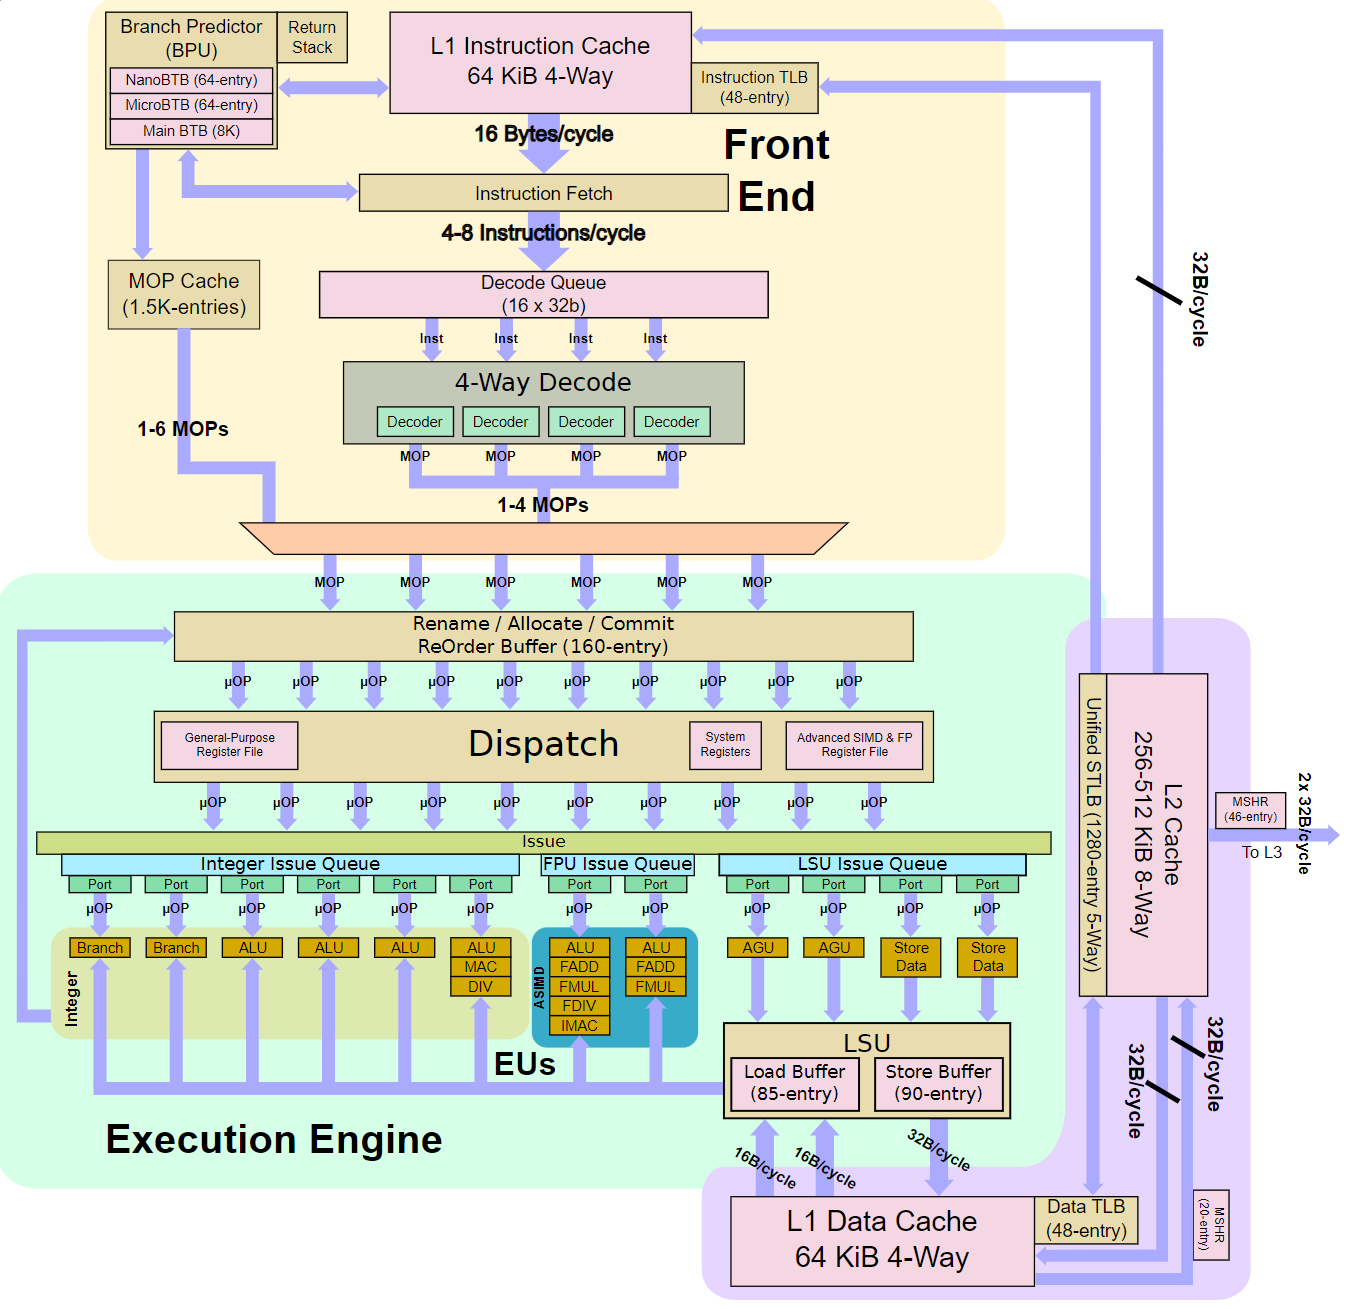
\includegraphics[width=161mm]{CortexA77}
        \label{cortexA77}
    \end{figure}

\subsubsection{Организация системы памяти}

    Процессор в современных мобильных системах встроен в так называемую SoC (System-on-chip --
    система на кристалле) систему -- электронная схема, которая выполняет цели компьютера
    и размещена на одной интегральной схеме. Таким образом, в такую систему встроены сразу процессор,
    таймеры, счётчики, интерфейсы для периферийных устройств, ОЗУ, ПЗУ и даже графический ускоритель.
    Именно таким образом устроены современные смартфоны, фотоаппараты, умные часы, элекронные книг
    и устройства схожего профиля.

    Одна из основных подсистем системы на кристалле -- подсистема памяти. Наиболее быстродействующими
    элементами памяти являются регистры ядра процессора, они же имеют наименьшее количество памяти,
    более высокую цену для производства и самую малую плотность расположения в электронной схеме.

    Учитывая малый объём возможного хранения данных с помощью регистров, а также
    что любая вычислительная система обладает локальностью (как по данным, так и по
    времени), почти всегда вводят дополнительные уровни памяти -- более дешёвые в производстве,
    имеющий больший объём и более высокую плотность ячеек хранения данных на электронной схеме.
    Более низкие уровни памяти являются кешами для более высоких.
    Таким образом, любая система имеет ОЗУ и кеши в качестве промежуточного хранилища данных
    (см. рис. \ref{CachePyramid}).

    Во всех современных мобильных системах в качестве ОЗУ используется LPDDR SDRAM
    (Low-Power Double Data Rate Synchronous Dynamic Random-Access Memory --
    динамическая оперативная память синхронного доступа с двойной скоростью передачи данных и
    с низким энергопотреблением). В дальнейшем для удобства будем использовать более простое
    обозначение для такой памяти -- DDR (Double Data Rate) память.

    Количество уровней кешей и объём их памяти напрямую зависят от требований к исполнению
    современных приложений и особенностей архитектуры мобильной системы,
    всегда являются компромиссом: с одной стороны, добавление дополнительного
    уровня кеша -- снижение вероятности обращения в DDR память (наиболее медленная память),
    а с другой -- введение постоянной дополнительной задержки при обращении в DDR, если данные
    в кешах отсутствуют.

    \begin{figure}[!h]
        \caption{Иерархия памяти в системе с 3-мя уровнями кешей}
        \centering
        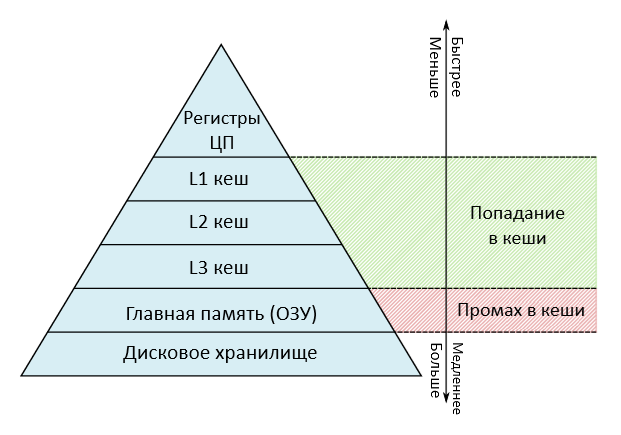
\includegraphics[width=116mm]{CachePyramidRU}
        \label{CachePyramid}
    \end{figure}

    Почти все современные процессоры имеют как минимум 2 уровня кешей. В системах на кристалле,
    как правило, последним (дополнительным) уровнем является системный кеш, который обычно
    не вносят в список уровней кешей процессора, так как он используется не только самим процессором,
    но также и различными периферийными устройствами, такими как графический ускоритель, ускоритель
    нейронных сетей и т.д.. Пример системы с 2-ся уровня кешей показан на рис. \ref{MulticoreCache}.

    \begin{figure}[!h]
        \caption{Пример иерархии кешей в многоядерном процессоре (отсутствуют кеш 3-его уровня
            и системный кеш)}
        \centering
        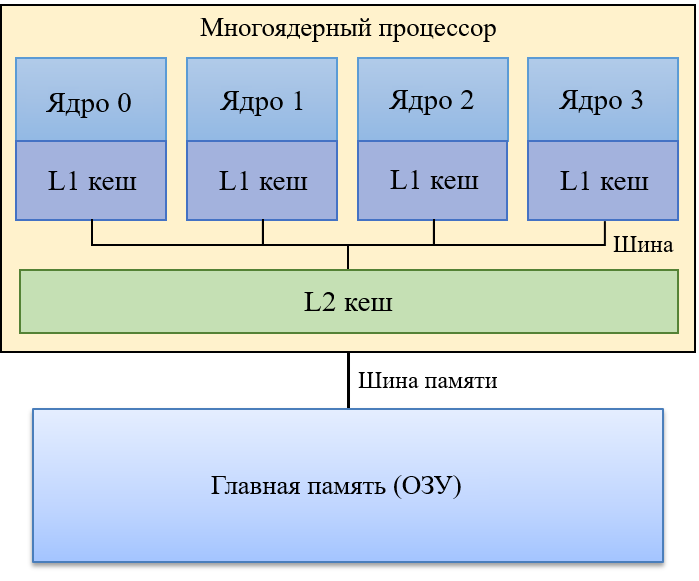
\includegraphics[width=95mm]{MulticoreCacheRU}
        \label{MulticoreCache}
    \end{figure}

    Каждое ядро процессора имеет собственный кеш инструкций и кеш данных, на которые для краткости
    ссылаются как на единый кеш 1-ого уровня. Остальные уровни кешей, как правило, являются объединёнными
    (для инструкций и данных).
    При промахе в кеш 1-ого уровня поиск данных происходит в кеше 2-ого уровня, при промахе
    в кеш 2-ого -- поиск в кеше 3-его (если таковой имеется), и так до тех пор, пока не произойдёт
    обращение в DDR память. (см. рис. \ref{MulticoreCache}).

    Как правило, кеш 2-ого уровня уникален для каждого ядра, хотя в некоторых гетерогенных системах
    кеш 2-ого уровня может использовать либо группой из 2-ух ядер в марках одного кластера, либо
    целиком всем кластером ядер (такое поведение характерно для современных энергоэффективных ядер).
    Кеш 3-его уровня всегда разделяется между всеми ядрами системы, как и системный кеш вместе с ОЗУ.

    ПЗУ, а также компоненты для долгосрочного хранения данных (диски, твёрдотельные накопители и др.)
    в данной работе рассматриваться не будут, под памятью будет иметься в виду только кеши процессора
    и ОЗУ.

\subsubsection{Латентность памяти и утилизация её пропускной способности} \label{lat_util_chapter}

    Начиная с этого момента и до коцна работы для краткости обозначения отношения величины
    затраченных тактов $cycles$ ядром процессора на исполнение количества инструкций $instrs$
    введём соотношение $cpi = cycles / instrs$.

    Для построения модели производительности ядра процессора, т.е. для правильного подсчёта утилизации
    ядра и наиболее энергоэффективного регулирования тактовых частот, важно учитывать не только
    структуру организации памяти в исследуемой системе, а также и динамические характеристики
    элементов такой системы. Наиболее важными характеристиками являются пропускная способность шин,
    соединяющих вычислительные подсистемы с подсистемами памяти, утилизация пропускной способности и
    латетность памяти -- промежуток времени между отправлением запроса на получение данных в память и
    между самим получением данных.

    Таким образом, кеши процессора и DDR память имеют свои собственные динамические характеристики,
    приведённые ранее. Как правило, низкие уровни кешей работают на той же тактовой частоте, что
    и само процессорное ядро, поэтому значение латентности таких кешей можно выразить через такты ядра
    процессора. Сложнее ситуация обстоит с более высокими уровнями кешей и DDR они имеют отдельные
    источники тактирования, значение латентности нельзя выразить через такты процессорного ядра,
    к тому же она зависит от утилизации пропускной способности шин, ведущих к этим элементам памяти,
    то есть от количества транзакций в единицу времени.

    Модель производительности ядра процессора требует учёта латентности памяти, поэтому
    необходимо рассмотреть существующие решения для её определения и/или возможного учёта в модели.

    Авторы статьи \cite{keramidas2010interval} предлагают 2 модели для учёта латентности памяти
    в рамках алгоритма регулирования тактовых частот. Первая модель разбивает такты ядра процессора
    на 2 компоненты: относящиеся к ожиданию транзакций памяти и относящиеся непосредственно к вычислительным
    блокам ядра процессора. Утверждается, что при изменении частоты ядра процессора изменяется только
    количество тактов, относящихся к памяти (тактовая частота которой независима от частоты ядра).
    На этом и основывается алгоритм регулирования частот, использующий перерасчёт времени
    исполнения через такты при различных частотах. Вторая модель является модификацией-улучшением
    первой модели: дополнительно предполагается, что в группе инструкций, которые обращаются в
    память подряд, следует учитывать только первую инструкцию в формуле для перерасчёта тактов,
    которые относятся к памяти, однако это требует наличие дополнительной информации на уровне кешей:
    среди всех промахов в кеши (т.е. обращений в следующий уровень памяти) следует учитывать только
    первые промахи среди группы промахов (промахов, находящихся на расстоянии порядка времени
    латентности обращения в вышележащие уровни памяти), что не поддерживается ни одним устройством
    на сегодняшний день.

    В работе также отмечается, что следует учитывать ROB в OoO процессорах: из тактов, относящихся к
    транзакциям памяти, следует вычесть ту часть тактов, которую тратит процессор на спекулятивное
    исполнение инструкций после инструкций-обращений в память.

    Подход использования аналитической формулы влияния утилизации пропускной способности памяти на
    её латентность рассматривается в статье \cite{clapp2015quantifying}: применяется
    метрика $cpi$, которая включает в себя слагаемые, связанные с тактами, потраченными
    на время ожидания транзакций-обращений в память. Авторы вводят понятие блокирующего фактора
    для латентности памяти: в зависимости от рабочей нагрузки при одинаковом количестве обращений в память
    влияние латентности на метрику ($cpi$) может меняться вплоть до десятка раз из-за параллельных
    обращений в память, что коррелирует с результатами работы \cite{keramidas2010interval}.
    При фиксированном блокирующем факторе значение $cpi$ зависит линейно от количества обращений
    в память в единицу инструкций.
    Таким образом, все рабочие нагрузки разделены на 2 вида: чувствительные к латентности (высокое
    значение блокирующего фактора) и чувствительные к пропускной способности (низкое значение
    блокирующего фактора).
    Однако данное исследование ограничивается рассмотрением обращений только в DDR память
    при фиксированных тактовых частотах всех устройств.

    Зависимость латентности памяти от утилизации пропускной способности представляет собой монотонную
    возрастающую функцию, которую можно положить константой при значениях утилизации, не сильно близкой
    к максимально возможной (\cite{david2011memory}), при приближении утилизации к своему максимуму
    значение латентности резко растёт.

    Таким образом, можно сделать основные выводы из существующих работ:
    \begin{enumerate}
        \item Чувствительность производительности к латентности памяти зависит от рабочей нагрузки и может
        быть очень низкой даже при большом количестве обращений в память (ОЗУ). Такая зависимость
        определяется уровнем параллелизма обращений в память.
        \item Латентность памяти является монотонной возрастающей функцией от утилизации пропускной
        способности, которую можно приближённо положить константой почти на всём интеравале утилизации;
        при стремлении утилизации к своему пределу происходит быстрый рост латентности до значений,
        на порядки превышающих значения при среднем уровне утилизации пропускной способности.
    \end{enumerate}

\subsection{Модель производительности ядра процессора} \label{model_chapter}

    Главной характеристикой производительности процессора является количество инструкций,
    исполняемых в еденицу времени -- чем больше это значение, тем быстрее исполняется рабочая
    нагрузка (приложение). Причём заданное количество инструкций исполняется за разное количество
    процессорных тактов, которые, в свою очередь, обратно пропорциональны времени исполнения
    этих инструкций.

    Пусть за время $\tau$ ядро процессора непрерывно исполняло инструкции и исполнило $instrs$
    инструкций за $cycles$ тактов при заданной тактовой частоте процессора $freq_{cpu}$.
    Тогда, очевидно, выполняется следующее соотношение:

    \begin{equation} \label{cycles_base}
        cycles = \frac{freq_{cpu}}{\tau}
    \end{equation}

    На практике чаще всего используют такие величины как $cpi = cycles / instrs$ и
    $ipc = instrs / cycles$ в качестве меры эффективности ядра процессора: чем выше/ниже значение
    $ipc$/$cpi$, тем эффективнее работа ядра процессора. Однако кроме типа процессорного ядра
    на эти значения также влияют тактовая частота самого ядра и тактовые частоты остальных компонент
    системы. Например, при повышении частоты ядра процессора величина $ipc$ либо остаётся такой же,
    если отсутствуют инструкции, связанные с обращением высокие уровни кешей или ОЗУ, либо уменьшается.

    За время $\tau$ процессор часть тактов тратит на исполнение инструкций непосредственно на
    ядерных блоках (в том числе вычислительных), а оставшуюся часть на ожидание операций,
    связанных с обращением в память (в кеши или оперативную память): обозначим эти величины
    $cycles_{cpu}$ и $cycles_{mem}$, тогда справедливо

    \begin{equation}
        cpi = \frac{cycles}{instrs} = \frac{cycles_{cpu}}{instrs} + \frac{cycles_{mem}}{instrs}
    \end{equation}

    Важно отметить, что $\frac{cycles_{cpu}}{instrs}$ -- значение $cpi$, если бы все обращения
    в кеши и оперативную память занимали 0 тактов, т.е. обрабатывались бы бесконечно быстро, а значит
    эта величина ограничивается снизу возможностями ядра процессора. Обозначим данное соотношение
    как $cpi_{cpu} \equiv \frac{cycles_{cpu}}{instrs}$.

    В свою очередь величина $cycles_{mem}$ характеризуется только лишь компонентами памяти,
    не зависящими от конвейера ядра процессора. Пусть, например, имеется 2 уровня кешей
    и ОЗУ, тогда время доступа к определённому уровню кеша характеризуется величиной $cycles_{L_{i}}$,
    представляющую собой латентность кеша (время задержки обращения), выраженную в ядерных тактах,
    где $i$ -- номер уровня кеша.

    После обращения в кеш возможны 2 ситуации: либо попадание к кеш, либо промах и обращение в
    следующий уровень кеша или ОЗУ, если кеша высшего уровня не осталось.
    Время доступа к оперативной памяти обозначим $cycles_{ram}$.

    Выразим времена доступа через такты ядра процессора и латентности, и введя обозначение
    $time^{-1}_{*} = \alpha_{*}^{par} \cdot n_{*} \cdot \frac{lat_{*}}{freq_{*}}$, где
    $\alpha_{*}^{par}$ --
    коэффициент параллелизма обращений в соответствующую компоненту памяти (см. \ref{lat_util_chapter}),
    $n_{*}$ -- количество таких обращений за время $\tau$, $lat_{*}$ -- средняя латентность
    одного обращения, выраженное не в ядерных тактах, а в собственных тактах компоненты памяти, получим:

    \begin{equation}
        cycles_{mem} = \left( time^{-1}_{L_1} + time^{-1}_{L_2} + time^{-1}_{ram} \right) \cdot freq_{cpu},
    \end{equation}

    \begin{equation}
        cpi = cpi_{cpu} + cpi_{mem},
    \end{equation}

    \begin{equation}
        cpi_{mem} = \left( \frac{n_{L_1}}{instrs} \cdot \frac{\alpha_{L_1}^{par} \cdot lat_{L_1}}{freq_{L_1}} +
        \frac{n_{L_2}}{instrs} \cdot \frac{\alpha_{L_2}^{par} \cdot lat_{L_2}}{freq_{L_2}} +
        \frac{n_{ram}}{instrs} \cdot \frac{\alpha_{ram}^{par} \cdot lat_{ram}}{freq_{ram}} \right) \cdot freq_{cpu},
    \end{equation}

    Заметим, что из формулы следует, что повышение тактовой частоты ядра процессора ведёт к
    увеличению $cpi$ и уменьшению $ipc$, а повышение тактовых частот кешей и оперативной памяти,
    наоборот, ведёт к уменьшению $cpi$ и увеличению $ipc$.

    Чаще всего уровни кешей, наиболее близкие к процессорному ядру, имеют такой же источник
    тактирования, что и процессорное ядро, т.е. такие кеши оперируют на тех же тактовых частотах,
    что и само ядро. Например, кеш первого уровня (кеши инструкций и данных) всегда оперирует с
    тактовой частотой ядра процессора ($freq_{L_1} = freq_{cpu}$), а значит формулу можно упростить
    до более простой:

    \begin{equation}
        cpi = cpi_{cpu} + \alpha_{L_1}^{par} \cdot lat_{L_1} \cdot \frac{n_{L_1}}{instrs} +
        \left( \frac{n_{L_2}}{instrs} \cdot \frac{\alpha_{L_2}^{par} \cdot lat_{L_2}}{freq_{L_2}} +
        \frac{n_{ram}}{instrs} \cdot \frac{\alpha_{ram}^{par} \cdot lat_{ram}}{freq_{ram}} \right) \cdot freq_{cpu}.
    \end{equation}

    Заметим, что можно ввести обозначение,
    $cpi_{cpu}^{L_1} = cpi_{cpu} + \alpha_{L_1}^{par} \cdot lat_{L_1} \cdot \frac{n_{L_1}}{instrs}$,
    полностью убрав из рассмотрения параметры обращения в кеш 1-ого уровня.

    \begin{equation}
        cpi = cpi_{cpu}^{L_1} +
        \left( \frac{n_{L_2}}{instrs} \cdot \frac{\alpha_{L_2}^{par} \cdot lat_{L_2}}{freq_{L_2}} +
        \frac{n_{ram}}{instrs} \cdot \frac{\alpha_{ram}^{par} \cdot lat_{ram}}{freq_{ram}} \right) \cdot freq_{cpu}.
    \end{equation}

    Так как в данной работе не предполагается регулирование тактовых частот устройств памяти, то
    обозначим для удобства величины $C_{*} = lat_{*} / freq_{*}$; также обозначим
    $npi_{*} = \frac{n_{*}}{instrs}$:

    \begin{equation}
        cpi = cpi_{cpu}^{L_1} +
        \left( \alpha_{L_2}^{par} \cdot C_{L_2} \cdot npi_{L_2} +
               \alpha_{ram}^{par} \cdot C_{ram} \cdot npi_{ram} \right) \cdot freq_{cpu}.
    \end{equation}

    Заметим, что величины $C_{L_2}$ и $C_{ram}$ не являются константами в общем случае, так как
    имеют смысл латентности обращения в память, которая зависит утилизации пропускной способности
    шины, ведущей к соответствующей компоненте памяти (см. \ref{lat_util_chapter}).

    Латентность оперативной памяти определяется как текущим уровнем утилизации этой памяти
    (шины, ведущей к памяти), так и особенностями обращения к ней (например, в случае DDR
    памяти, где элементарными ячейками являются банки данных, состоящие из строк и столбцов,
    существует кеш строки, который значительно влияет на скорость обращения
    к ячейке памяти, т.е. локальность обращения к ячейкам DDR памяти очень важна).

    В качестве упрощения примем $\alpha_{L_2}^{par} = \alpha_{ram}^{par} \equiv \alpha^{par}$, полагая,
    что коэффициенты параллелизма обращений в кеш последнего уровня (2-ого) и ОЗУ коррелируют.

    Финальная формула:

    \begin{equation} \label{cpi_formula}
        cpi = cpi_{cpu}^{L_1} + \alpha^{par} \cdot
        \left( C_{L_2} \cdot npi_{L_2} + C_{ram} \cdot npi_{ram} \right) \cdot freq_{cpu}.
    \end{equation}

    У описываемой модели есть ряд преимуществ, которые делают её лучше аналогичных моделей:
    \begin{enumerate}
        \item Явно введён коэффициент параллелизма обращений в память в $\alpha^{par}$, который можно
        регулировать динамически во время регулирования тактовой частоты ядра процессора.
        \item Такие величины, как $npi_{L_2}$ и $npi_{ram}$ можно получить в режиме реального времени
        практически во всех современных устройствах, в том числе в устройствах с архитектурой ARM64,
        которая используется в данной работе.
        \item Величины $C_{L_2}$ и $C_{ram}$ можно положить константами и вычислить заранее, так как
        в случае увеличения латентности памяти при приближении пропускной способности шин к максимальным
        значениям ответственность за увеличение этих коэффициентов неявно можно переложить на параметр
        $\alpha^{par}$, который уже предполагает дамическое регулирование.
        \item Величина $cpi_{cpu}^{L_1}$ не предполагает явного вычисления через другие формулы;
        достаточно знать все остальные коэффициенты, тогда эту величину можно найти по формуле
        \eqref{cpi_formula}, далее использовать её для оценки $cpi$ на других тактовых частотах.
        \item В случае физического ядра, разделённого на 2 виртуальных (так называемый
        SMT - Simultaneous multithreading), по-прежнему можно пользоваться формулой выше, т.к.
        становится неважно, как именно виртуальные ядра разделяют между собой процессорные блоки
        и как именно они взаимодействуют с кешом первого уровня -- эти аспекты учитываются
        в формуле в коэффициенте $cpi_{cpu}^{L_1}$ и не требуют дополнительных вычислений.
    \end{enumerate}

    Таким образом, для применения модели необходимо иметь:
    \begin{enumerate}
        \item Значения $C_{L_2}$ и $C_{ram}$, вычисленные заранее.
        \item Алгоритм регулирования параметра $\alpha^{par}$.
        \item Возможность измерения величин $cpi$, $npi_{L_2}$ и $npi_{ram}$ в режиме реального времени.
    \end{enumerate}

\subsection{Модель производительности ядра процессора применительно к архитектуре ARM} \label{model_counters}

    Рассмотрим способ применения описанной выше модели в случае архитектуры ARM64.
    Требуется уметь измерять величины $cpi$, $npi_{L_2}$ и $npi_{ram}$. Величина $npi_{L_2}$
    может быть найдена через количество промахов в кеш 1-ого уровня, а величина $npi_{ram}$ --
    через количество промахов в кеш 2-ого уровня (последний уровень).

    Следует воспользоваться следующими счётчиками микроархитектурных событий (\cite{ArmPMUjson}):
    \begin{enumerate}
        \item $CPU\_CYCLES$ -- количество тактов ядра процессора;
        \item $INST\_RETIRED$ -- количество исполненных инструкций;
        \item $L1I\_CACHE\_REFILL$ -- количество перезаполнений кеш-линий с инструкциями в кеше
        инструкций 1-ого уровня из-за промахов в этот кеш при чтении инструкции;
        некешируемые промахи в кеш и операции синхронизации кешей не считаются;
        \item $L1D\_CACHE\_REFILL$ -- количество перезаполнений кеш-линий с данными в кеше данных
        1-ого уровня из-за промахов в этот кеш;
        некешируемые промахи в кеш и операции синхронизации кешей не считаются;
        \item $L2D\_CACHE\_REFILL$ -- работает как сумма счётиков $L1D\_CACHE\_REFILL$ \\ и
        $L1I\_CACHE\_REFILL$, но применительно ко 2-ому уровню кеша.
    \end{enumerate}

    Заметим, что счётчик микроархитектурных событий $L2I\_CACHE\_REFILL$, как правило, не реализуется
    в ядрах ARM64, т.к. кеши 2-ого и выше уровней всегда объединённые (хранят как инструкции, так и данные).

    В счётчиках типа $*_\_CACHE\_REFILL$ существует очень важный нюанс, не оговорённый
    в спецификациях счётчиков микроархитектурных событий компании ARM Ltd., но упоминаемый
    в иных документах (см. \cite{ArmPerfAnalyses}): в платформах архитектуры ARM не существует счётчиков,
    которые считают промахи в кеши, вместо них используются счётчики, считающие
    количество перезаполнений кеш-линий (кешами более выского уровня или оперативной памятью).
    Возможна ситуация, когда один промах в кеш вызывает несколько перезаполнений кеш-линий
    (например, если промах случился по адресу, по которому значение пересекает 2 соседние кеш-линии),
    или наоборот: несколько промахов в кеш могут быть разрешены благодаря одному перезаполнению кеш-линии.

    Таким образом, величины $cpi$, $npi_{L_2}$ и $npi_{ram}$ можно найти через счётчики микроархитектурных
    событий следующим образом:
    \begin{equation}
        cpi = \frac{CPU\_CYCLES}{INST\_RETIRED},
    \end{equation}

    \begin{equation}
        npi_{ram} = \frac{L2D\_CACHE\_REFILL}{INST\_RETIRED}.
    \end{equation}

    \begin{equation}
        npi_{L_2} = \frac{L1I\_CACHE\_REFILL + L1D\_CACHE\_REFILL}{INST\_RETIRED} - npi_{ram},
    \end{equation}

    Заметим, что чаще всего в современных мобильных системах на архитектуре ARM64 после последнего
    уровня процессорного кеша располагают дополнительный кеш -- системный кеш,
    который предназначен для периферийных устройств и находится между оперативной памятью и процессором.
    Он может быть как больше по размеру, чем последний уровень процессорного кеша, так и меньше.
    Наличие системного кеша ведёт к тому, что для определения значения $n_{ram}$ недостаточно
    воспользоваться счётчиками, описанными выше; единственным счётчиком микроархитектурных событий,
    который может подойти в данном случае, является $LL\_CACHE\_MISS\_RD$ -- данный счётчик считает
    количество перезаполнений кеш-линий в кеш последнего уровня, в которых данные взяты из оперативной памяти,
    либо из другого чипа, либо из соседнего процессорного кластера с использованием технологии Intercluster peering.

    Согласно документации ARM64 (\cite{ArmPerfAnalyses}), если счётчик $LL\_CACHE\_MISS\_RD$ не реализован,
    то есть бит $EXTLLC$ в регистре $CPUECTLR$ выставлен в ноль, то значения $LL\_CACHE\_MISS\_RD$
    будут совпадать со значениями $L2D\_CACHE\_REFILL$ (в случае процессора с 2-мя уровнями кешей).
    В случае наличия системного кеша игнорирование этого счётчика может заметно ухудшит
    работу модели, однако в данной работе наличие системного кеша не предполагается, так что данный
    счётчик будет проигнорирован.

\subsection{Способ применения модели производительности ядра процессора в ядре Linux}

    В этой главе будут использоваться термины утилизации, введённые в главе \ref{linux_util}.

    Для применения описанной ранее модели производительности, необходимо разработать формулы для
    вычислений следующих значений:
    \begin{enumerate}
        \item Утилизация потока исполнения на основе утилизации ядерного времени этим потоком за
        фиксированный промежуток времени.
        \item Тактовая частота, которую необходимо выставить, на основе значения подсчитанной
        утилизации (или утилизаций за несколько промежутков времени).
        \item Коэффициент параллелизма обращений в память $\alpha^{par}$ для следующего промежутка
        времени.
    \end{enumerate}

\subsubsection{Вычисление утилизации потока исполнения}

    По определению утилизация потока исполнения -- часть ёмкости производительности,
    использованной при заданной утилизации ядерного времени, а
    ёмкость производительности -- количество исполненных инструкций в единицу времени при заданной
    тактовой частоте при условии максимальной утилизации ядерного времени (см. \ref{linux_util}).

    Пусть $\tau$ -- величина промежутка времени, за которую будет подсчитана утилизация потока исполнения.
    Рассмотрим для упрощения только 1 ядро процессора, тактовая частота которого фиксированна.
    Тогда, согласно определениям, приведённым выше, справедливо

    \begin{equation}
        util = 1024 \cdot \frac{\Delta t}{\tau} \cdot \frac{instrs / s}{(instrs / s) |_{freq_{cpu} = freq_{cpu}^{max}}} =
            1024 \cdot \frac{\Delta t}{\tau} \cdot \frac{instrs}{(instrs) |_{freq_{cpu} = freq_{cpu}^{max}}}
    \end{equation}
    где $\Delta t$ -- время активной работы ядра процессора, $\frac{\Delta t}{\tau}$ -- утилизация ядерного
    времени, $instrs / s$ -- количество выполняемых инструкций в единицу времени при заданной тактовой
    частоте, а $(instrs / s) |_{freq_{cpu} = freq_{cpu}^{max}}$ -- максимально возможное для
    рассматриваемой рабочей нагрузки значение выполняемых инструкций в единицу времени, достигаемое
    повышением тактовой частоты ядра до своего максимального значения.

    % Заметим, что величины $instrs$ и $(instrs) |_{freq_{cpu} = freq_{cpu}^{max}}$ рассматриваются для одинакового
    % промежутка времени, и $(instrs) |_{freq_{cpu} = freq_{cpu}^{max}}$ несёт за собой смысл количества инструкций,
    % которые были бы исполнены ядром процессора за то же количество тактов, на при максимальной тактовой частоте.
    % Значит справедливо выражение

    % \begin{equation}
    %     util = 1024 \cdot \frac{\Delta t}{\tau} \cdot \frac{ipc}{(ipc) |_{freq_{cpu} = freq_{cpu}^{max}}}
    % \end{equation}

    Заметим, что

    \begin{equation}
        instrs / s = \frac{instrs}{cycles} \cdot \frac{cycles}{s} = \frac{1}{cpi} \cdot freq_{cpu} =
        \frac{freq_{cpu}}{cpi},
    \end{equation}
    тогда формула утилизации принимает следующий вид:

    \begin{equation} \label{util_general_cpi}
        util = 1024 \cdot \frac{\Delta t}{\tau} \cdot \frac{\frac{freq_{cpu}}{cpi}}{\left( \frac{freq_{cpu}}{cpi} \right)
            \bigg|_{freq_{cpu} = freq_{cpu}^{max}}} = 1024 \cdot \frac{\Delta t}{\tau} \cdot
            \frac{freq_{cpu}}{freq_{cpu}^{max}} \cdot \frac{cpi |_{freq_{cpu} = freq_{cpu}^{max}}}{cpi}.
    \end{equation}

    Возникший множитель $\frac{cpi |_{freq_{cpu} = freq_{cpu}^{max}}}{cpi}$ явно предполагался равным единице
    в решении, описанном в главе \ref{linux_util}, в формуле \eqref{util_linux_formula}.

    Подставив формулу модели производительности \eqref{cpi_formula} в формулу \eqref{util_general_cpi},
    а также обозначив $lat_{gen} = \alpha^{par} \cdot \left( C_{L_2} \cdot npi_{L_2} + C_{ram} \cdot npi_{ram} \right)$,
    получим:

    \begin{equation} \label{util_formula_final}
        util = 1024 \cdot \frac{\Delta t}{\tau} \cdot \frac{freq_{cpu}}{freq_{cpu}^{max}} \cdot
            \frac{cpi_{cpu}^{L_1} + lat_{gen} \cdot freq_{cpu}^{max}}
                 {cpi_{cpu}^{L_1} + lat_{gen} \cdot freq_{cpu}}.
    \end{equation}

    В формуле \eqref{util_formula_final} предполагается использовать значения $cpi_{cpu}^{L_1}$ и $lat_{gen}$,
    посчитанные в конце предыдущего промежутка времени для расчёта утилизации за текущий промежуток времени.

    Если $cpi_{cpu}^{L_1} \ll lat_{gen} \cdot freq_{cpu}$, то

    \begin{equation}
        util \approx 1024 \cdot \frac{\Delta t}{\tau} \cdot \frac{freq_{cpu}}{freq_{cpu}^{max}} \cdot
            \frac{lat_{gen} \cdot freq_{cpu}^{max}} {lat_{gen} \cdot freq_{cpu}} =
            1024 \cdot \frac{\Delta t}{\tau},
    \end{equation}
    то есть утилизация перестаёт зависеть от частоты ядра процессора,
    что и следовало ожидать.

    Если $cpi_{cpu}^{L_1} \gg lat_{gen} \cdot freq_{cpu}$, то есть вклад тактов, затраченных на ожидание
    обращений в память, мал по сравнению с остальным числом тактов, то

    \begin{equation}
        util \approx 1024 \cdot \frac{\Delta t}{\tau} \cdot \frac{freq_{cpu}}{freq_{cpu}^{max}} \cdot
            \frac{cpi_{cpu}^{L_1}} {cpi_{cpu}^{L_1}} = 1024 \cdot \frac{\Delta t}{\tau} \cdot
            \frac{freq_{cpu}}{freq_{cpu}^{max}},
    \end{equation}
    то есть формула совпадает с формулой \eqref{util_linux_formula}, использованной в ядре Linux.

    Рассмотрим теперь более общий случай, когда тактовая частота в одном промежутке времени $\tau$
    не фиксирована, как предполагалось до этого (см. формулу \eqref{util_formula_final}), а может
    изменяться (например, из-за того, что в ядерном кластере соседнее ядро решило повысить тактовую
    частоту). Пусть $i$ -- номер подынтеравала, на котором процессор был активен и его тактовая
    частота равнялась $freq_{cpu, i}$.

    \begin{equation}
        util = 1024 \cdot \frac{\Delta t}{\tau} \cdot
            \frac{\langle instrs / s \rangle_t }{ \langle (instrs / s) |_{freq_{cpu, i} = freq_{cpu}^{max}} \rangle_t},
            \; \Delta t = \sum \limits_i \Delta t_i.
    \end{equation}

    \begin{equation}
        util = 1024 \cdot \frac{\sum \limits_i \Delta t_i}{\tau} \cdot
            \frac{\frac{1}{\tau} \sum \limits_i (instrs / s)_i \cdot \Delta t_i}
                 {\frac{1}{\tau} \sum \limits_i (instrs / s)_i \cdot \Delta t_i |_{freq_{cpu, i} = freq_{cpu}^{max}}} =
    \end{equation}

    \begin{equation*}
        = 1024 \cdot \frac{\Delta t}{\tau} \cdot
        \frac{\sum \limits_i \frac{instrs_i}{\Delta t_i} \cdot \Delta t_i}
             {\sum \limits_i (\frac{instrs_i}{\Delta t_i} \cdot \Delta t_i) |_{freq_{cpu, i} = freq_{cpu}^{max}}} =
        1024 \cdot \frac{\Delta t}{\tau} \cdot
        \frac{\sum \limits_i instrs_i}
             {\sum \limits_i instrs_i |_{freq_{cpu, i} = freq_{cpu}^{max}}}.
    \end{equation*}

    \begin{equation}
        \frac{instrs_i |_{freq_{cpu, i} = freq_{cpu}^{max}}}{instrs_i} =
            \frac{(\frac{freq_{cpu}}{cpi}) |_{freq_{cpu} = freq_{cpu}^{max}}}{\frac{freq_{cpu, i}}{cpi_i}} =
            \frac{freq_{cpu}^{max}}{freq_{cpu, i}} \cdot \frac{cpi_i}{cpi |_{freq_{cpu, i} = freq_{cpu}^{max}}} =
    \end{equation}

    \begin{equation*}
        = \frac{freq_{cpu}^{max}}{freq_{cpu, i}} \cdot \frac{cpi_{cpu}^{L_1} + lat_{gen} \cdot freq_{cpu}^{max}}
            {cpi_{cpu}^{L_1} + lat_{gen} \cdot freq_{cpu, i}},
    \end{equation*}
    откуда можно получить финальную для утилизации:

    \begin{equation} \label{util_sum_final}
        util = 1024 \cdot \frac{\Delta t}{\tau} \cdot \frac{\sum \limits_i instrs_i}
            {\sum \limits_i instrs_i \cdot \frac{freq_{cpu}^{max}}{freq_{cpu, i}} \cdot
            \frac{cpi_{cpu}^{L_1} + lat_{gen} \cdot freq_{cpu}^{max}}{cpi_{cpu}^{L_1} + lat_{gen} \cdot freq_{cpu, i}}}.
    \end{equation}

    Важно отметить, что хотя суммирование проводится в течение одного промежутка времени $\tau$,
    значение $cpi_{cpu}^{L_1}$ всё ещё считается в конце предыдущего промежутка времени в
    предположении, что оно останется таким же в текущем промежутке, так же как и величина $lat_{gen}$
    (после регулирования параметра $\alpha^{par}$, подробнее в главе \ref{alpha_regul}).

    Однако, теперь расчёт $cpi_{cpu}^{L_1}$ в конце каждого промежутка не такой тривиальный: в
    каждом подынтервале $i$ текущего промежутка времени необходимо сделать следующее:

    \begin{equation}
        cpi_i = cpi_{cpu, i}^{L_1} + lat_{gen, i} \cdot freq_{cpu, i} \Rightarrow
            cycles_i = cycles_{cpu, i}^{L_1} + lat_{gen, i} \cdot freq_{cpu, i} \cdot instrs_i \Rightarrow
    \end{equation}

    \begin{equation*}
        \Rightarrow cycles_{cpu, i}^{L_1} = cycles_i - lat_{gen, i} \cdot freq_{cpu, i} \cdot instrs_i \Rightarrow
        cpi_{cpu}^{L_1} := \frac{\sum \limits_i cycles_{cpu, i}^{L_1}}{\sum \limits_i instrs_i}, \; \text{т.е.}
    \end{equation*}

    \begin{equation} \label{cpi_l1_sum}
        cpi_{cpu}^{L_1} := \frac{\sum \limits_i cycles_i - \alpha^{par} \cdot \left( C_{L_2} \cdot n_{L_2, i} +
            C_{ram} \cdot n_{ram, i} \right) \cdot freq_{cpu, i}}{\sum \limits_i instrs_i},
    \end{equation}
    именно такое значение будет посчитано в конце текущего промежутка времени и использованного в следующем
    промежутке по формуле \eqref{util_sum_final}.

    Вдобавок отметим, что
    \begin{equation} \label{latency_sum}
        lat_{gen} := \alpha^{par} \cdot \frac{\sum \limits_i C_{L_2} \cdot n_{L_2, i} + C_{ram} \cdot n_{ram, i}}
            {\sum \limits_i instrs_i}.
    \end{equation}

\subsubsection{Выбор тактовой частоты ядра процессора}

    Выбор тактовой частоты основывается на посчитанной утилизации по формуле \eqref{util_sum_final}.
    Предположим, что за промежуток времени $\tau$ ядро процессора было активным время $\Delta t < \tau$.
    Смысл регулирования тактовой частоты заключается в том, что если $\Delta t$ не сильно близко к
    значению $\tau$, то тактовую частоту можно понизить так, чтобы $\Delta t$ всё ещё оставалось меньшим
    величины $\tau$, т.е. чтобы приложение всё ещё успевало выполнять требуемую работу.

    Если $\Delta t > \tau$ на текущей тактовой частоте, то, как минимум, тактовую частоту требуется повышать,
    но насколько повышать -- аналитически выявить невозможно, поэтому предлагается следующий алгоритм:
    если такая ситуация произошла только 1 раз, тактовая частота повышается на $n$ уровней (возможные
    значения тактовых частот всегда дискретны), если после этого она произошла ещё раз, то тактовая частота
    повышается до максимально возможного значения.

    Чтобы ситуация $\Delta t > \tau$ происходила более редко, предлагается так же, как и в решениях,
    описанных в главе \ref{linux_util}, выставлять тактовую частоту с запасом по утилизации, то есть
    условие выбора тактовой частоты $\Delta t < \tau$ заменяется на $\Delta t < \gamma \cdot \tau$,
    $\gamma < 1$. Часто выбирают $\gamma = 0.8$, но выбор такого значения лучше подбирать под
    конкретные рабочих нагрузок (приложения).

    Величина $\Delta t$ в условии $\Delta t < \gamma \cdot \tau$ выражается через параметры модели
    производительности, посчитанной утилизации и тактовой частоты процессора, откуда и извлекается минимальное
    значение тактовой частоты для соблюдения данного условия (неравенства). Тактовая частота находится из
    предположения, что в следующий промежуток времени $\tau$ утилизация $util$ приложения останется
    такой же (как посчитанное значение), а тактовая частота выбирается полностью на весь промежуток времени,
    поэтому необходимо использовать формулу утилизации \eqref{util_formula_final}:

    \begin{equation}
        util = 1024 \cdot \frac{\Delta t}{\tau} \cdot \frac{freq_{cpu}}{freq_{cpu}^{max}} \cdot
            \frac{cpi_{cpu}^{L_1} + lat_{gen} \cdot freq_{cpu}^{max}}
                 {cpi_{cpu}^{L_1} + lat_{gen} \cdot freq_{cpu}}, \; \frac{\Delta t}{\tau} < \gamma \Rightarrow
    \end{equation}

    \begin{equation}
        \Rightarrow \frac{util}{1024} \cdot \frac{freq_{cpu}^{max}}{freq_{cpu}} \cdot
        \frac{cpi_{cpu}^{L_1} + lat_{gen} \cdot freq_{cpu}}
             {cpi_{cpu}^{L_1} + lat_{gen} \cdot freq_{cpu}^{max}} < \gamma \; (\gamma < 1) \Rightarrow
    \end{equation}

    \begin{equation} \label{optimal_cpufreq}
        \Rightarrow freq_{cpu} > \frac{\tilde{util} \cdot freq_{cpu}^{max} \cdot cpi_{cpu}^{L_1}}
        {cpi_{cpu}^{L_1} + lat_{gen} \cdot freq_{cpu}^{max} \cdot (1 - \tilde{util})}, \;
        \text{где} \; \tilde{util} = \frac{util}{1024 \cdot \gamma}.
    \end{equation}

    Если $\tilde{util} > 1$, т.е. $freq_{cpu} > \tilde{util} \cdot freq_{cpu}^{max} > freq_{cpu}^{max}$,
    а если $util \rightarrow 0$, то $freq_{cpu} > 0$, то есть граничные случаи удовлетворяют определению
    утилизации.

    Таким образом, тактовая частота ядра процессора на следующий промежуток времени выбирается исходя
    из формулы \eqref{optimal_cpufreq}. Значение $\alpha^{par}$ берётся после этапа регулирования
    (подробнее в главе \ref{alpha_regul}) в конце текущего промежутка времени, а величины
    $cpi_{cpu}^{L_1}$ и $lat_{gen}$ считаются по формулам \eqref{cpi_l1_sum} и \eqref{latency_sum}
    прямо перед расчётом тактовой частоты после этапа регулирования $\alpha^{par}$.

\subsubsection{Алгоритм регулирования коэффициента параллелизма обращений в память} \label{alpha_regul}

    Утилизация рассчитывается суммированием слагаемых во множителях по формуле \eqref{util_sum_final}
    в течение всего промежутка времени на основе параметров, посчитанных в конце предыдущего промежутка
    времени; тактовая частота вычисляется из посчитанного значения утилизации и параметров, посчитанных
    уже в конце текущего промежутка времени. Одним единственным параметром, регулирование которого должна
    осуществляться вшеним способом, является $\alpha^{par}$.

    В начале иницилизации модели параметр $\alpha^{par} := 1$ полагается равным единице. Далее в конце
    каждого промежутка времени осуществляется его регулирование.

    Чтобы избежать колебательных процессов и расхождений параметра $\alpha^{par}$, предлагается
    ввести агрегацию таких параметров за несколько промежутков времени подряд -- вычисляться будет
    новое значение $\alpha^{par}$, но применяться в формулах агрегированное за несколько последних
    промежутков времени после добавления нового значения. Одной из наиболее эффективных и простых
    эвристик является использование экспоненциально взвешенного скользящего среднего значения за
    последние $n$ промежутков; предлагается выбрать $n = 5$, аналогично значению, выбранному в алгоритме
    подсчёта утилизации WALT (см. главу \ref{linux_util}).

    Само значение коэффициента $\alpha^{par}$, которое будет использовано в экспоненциально взвешенном
    скользящем среднем значении, предлагается искать через сравнение величин $cpi_{cpu}^{L_1}$,
    подсчитанных за предыдущий и за текущие промежутки времени. Во-первых, это компонента является
    зависимой от параметра $\alpha^{par}$ в формуле \eqref{cpi_l1_sum}. Во-вторых, она не требует
    знаний и тактовых частот, которые были выставлены на ядре процессора.

    В любом случае параметр $\alpha^{par}$ возможно регулировать лишь в случае изменений тактовых частот
    для получения обратной связи, поэтому требуется некоторый период релаксации для установления
    подходящего значения $\alpha^{par}$ для рабочей нагрузки (приложения).

    Идея заключается в следующем наблюдении: если значение $cpi_{cpu}^{L_1}$ выросло по сравнению
    со значением в предыдущий промежуток времени, то, скорее всего (т.к. нет гарантии установления
    источника изменения этой величины), исходя из формулы \eqref{cpi_l1_sum}, параметр $\alpha^{par}$
    оказался меньше своего реального значения и требует корректировки в сторону повышения.
    Поэтому новое значение коэффициента параллелизма для $j$-ого промежутка времени можно положить равным

    \begin{equation}
        \alpha^{par}_j := \alpha^{par}_{j - 1} \cdot \frac{cpi_{cpu, j}^{L_1}}{cpi_{cpu, j - 1}^{L_1}},
    \end{equation}
    где $cpi_{cpu, j}^{L_1}$ -- значение $cpi_{cpu}^{L_1}$ за $j$-ый промежуток.

    Заметим, что при таком подходе в случае некорректного значения $\alpha^{par}$ ошибка компенсируется
    использованием экспоненциально взвешенного скользящего среднего значения. Для $j$-ого промежутка
    в результате будет использован следующий коэффициент параллелизма:

    \begin{equation}
        \alpha^{par}_{avg} = \frac{1}{n} \sum \limits_{i = 0}^{n - 1} \beta^{i} \alpha^{par}_{j - i},
        \; 0 < \beta < 1.
    \end{equation}

% \subsection{Реализация модели в планировщике ядра Linux}

%     TBD

\newpage
